% Generated by scripts/generate_paper_figures.py — do not edit by hand.
% Source: experiments/2026-07-05_injection_exp2/out/results.json
% Requires \usepackage{pgfplots} and \pgfplotsset{compat=1.18}.
\begin{figure*}[t]
\centering
\pgfplotsset{
  detbar/.style={
    xbar, width=0.47\textwidth, height=4.1cm,
    xmin=0, xmax=1.19, xtick={0,0.25,0.5,0.75,1.0},
    bar width=7pt, y=0.52cm,
    axis lines*=left, axis line style={gray!50},
    xmajorgrids, grid style={gray!22, line width=0.4pt},
    tick label style={font=\scriptsize},
    xlabel style={font=\scriptsize, yshift=2pt},
    title style={font=\small, align=center, yshift=1pt},
    error bars/x dir=both, error bars/x explicit,
    error bars/error bar style={gray!70!black, line width=0.6pt},
    error bars/error mark options={rotate=90, mark size=1.4pt, gray!70!black},
    ytick={0,1,2,3,4,5},
    enlarge y limits={abs=0.5},
    clip=false,
  },
}
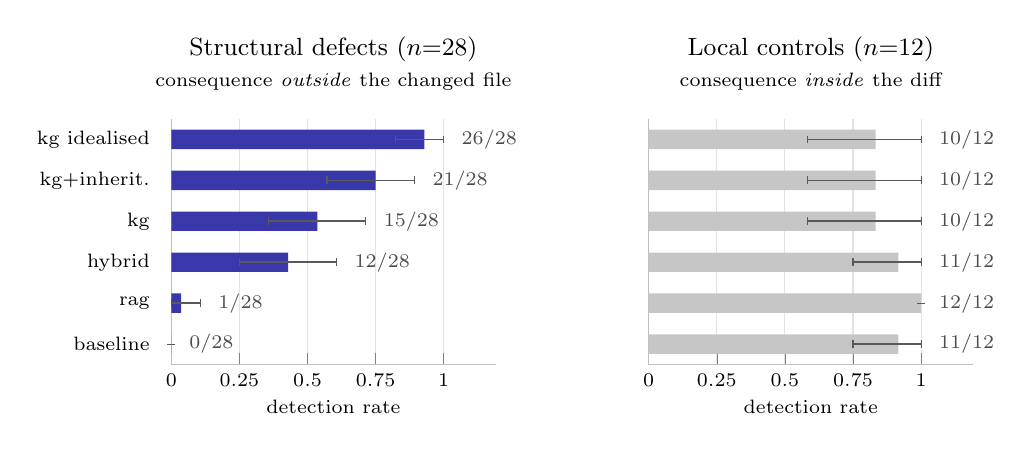
\begin{tikzpicture}
\begin{axis}[detbar,
    yticklabels={baseline,rag,hybrid,kg,kg+inherit.,kg idealised},
    ytick style={draw=none},
    xlabel={detection rate},
    title={Structural defects ($n{=}28$)\\\scriptsize consequence \emph{outside} the changed file},
  ]
  \addplot+[draw=none, fill=blue!58!black!78] plot coordinates {
        (0.0000,0) +- (0.0000,0) -= (0.0000,0)
        (0.0357,1) +- (0.0714,0) -= (0.0357,0)
        (0.4286,2) +- (0.1786,0) -= (0.1786,0)
        (0.5357,3) +- (0.1786,0) -= (0.1786,0)
        (0.7500,4) +- (0.1429,0) -= (0.1786,0)
        (0.9286,5) +- (0.0714,0) -= (0.1071,0)
  };
      \node[anchor=west,font=\scriptsize,gray!60!black] at (axis cs:0.0300,0) {0/28};
      \node[anchor=west,font=\scriptsize,gray!60!black] at (axis cs:0.1371,1) {1/28};
      \node[anchor=west,font=\scriptsize,gray!60!black] at (axis cs:0.6371,2) {12/28};
      \node[anchor=west,font=\scriptsize,gray!60!black] at (axis cs:0.7443,3) {15/28};
      \node[anchor=west,font=\scriptsize,gray!60!black] at (axis cs:0.9229,4) {21/28};
      \node[anchor=west,font=\scriptsize,gray!60!black] at (axis cs:1.0300,5) {26/28};
\end{axis}
\begin{axis}[detbar, at={(0.5\textwidth,0)}, anchor=south west,
    yticklabels={,,},
    ytick style={draw=none},
    xlabel={detection rate},
    title={Local controls ($n{=}12$)\\\scriptsize consequence \emph{inside} the diff},
  ]
  \addplot+[draw=none, fill=gray!45] plot coordinates {
        (0.9167,0) +- (0.0833,0) -= (0.1667,0)
        (1.0000,1) +- (0.0000,0) -= (0.0000,0)
        (0.9167,2) +- (0.0833,0) -= (0.1667,0)
        (0.8333,3) +- (0.1667,0) -= (0.2500,0)
        (0.8333,4) +- (0.1667,0) -= (0.2500,0)
        (0.8333,5) +- (0.1667,0) -= (0.2500,0)
  };
      \node[anchor=west,font=\scriptsize,gray!60!black] at (axis cs:1.0300,0) {11/12};
      \node[anchor=west,font=\scriptsize,gray!60!black] at (axis cs:1.0300,1) {12/12};
      \node[anchor=west,font=\scriptsize,gray!60!black] at (axis cs:1.0300,2) {11/12};
      \node[anchor=west,font=\scriptsize,gray!60!black] at (axis cs:1.0300,3) {10/12};
      \node[anchor=west,font=\scriptsize,gray!60!black] at (axis cs:1.0300,4) {10/12};
      \node[anchor=west,font=\scriptsize,gray!60!black] at (axis cs:1.0300,5) {10/12};
\end{axis}
\end{tikzpicture}
\caption{Defect detection by arm, with 95\% bootstrap confidence intervals and
raw counts. Left: defects whose consequence provably lies outside the changed
file. The diff-only baseline detects none, embedding retrieval detects one,
and graph context detects fifteen; the idealised resolver shows how much of
the remaining gap belongs to graph construction rather than to the model.
Right: the placebo band, where the defect is visible in the diff and no arm
should gain from added context --- and none does. The contrast between the two
panels is what distinguishes a structural capability from a context-volume
artefact.}
\label{fig:detection-ladder}
\end{figure*}
